\chapter{Literature Review}
% Main Gist 
% - History of FHR reactor type and why there is a renewed interest in this
%   reactor type (start ups, labs etc.)
% - Past applications of AI to nuclear reactor design. 
% Structure 
% - Fluoride-Salt-Cooled High-Temperature Reactor (why salt cooled triso fuelled 
%   reactors are cool)
%   - FHR Modeling Challenges (why benchmark exists)
%   - Description of benchmark
% - Artificial Intelligence Applications to Nuclear Reactor Design Optimization
%   - Past work 
%   - Classical vs Evolutionary methods 

\section{Fluoride-Salt-Cooled High-Temperature Reactor}
The \gls{FHR} is a reactor concept introduced in 2012 that uses high-temperature 
coated-particle fuel and a low pressure liquid fluoride-salt coolant 
\cite{forsberg_fluoride-salt-cooled_2012,facilitators_fluoride-salt-cooled_2013}.
\gls{FHR} technology combines the best aspects of \gls{MSR} and \gls{VHTR} 
(or \gls{HTGR}) technologies. 
Molten fluoride salts as working fluids for nuclear reactors have been explored 
since the 1960s and are desirable because of the salts' high-temperature 
performance and overall chemical stability \cite{scarlat_design_2014}.  
Using molten salts for reactor coolant introduces inherent safety compared 
to water due to the salts' high boiling temperature and high volumetric 
heat capacity, eliminating the risk of coolant boiling off, resulting in 
fuel elements overheating \cite{ho_molten_2013}. 
The leading candidate coolant salt is the fluoride salt Li$_2$BeF$_4$ (FLiBe), 
which remains liquid without pressurization up to 1400 $^{\circ}$C and a larger 
$\rho C_p$ than water \cite{ho_molten_2013,forsberg_fluoride-salt-cooled_2012}. 
\glspl{FHR} are favorable compared to a liquid fuel reactor, such as
\gls{MSR} systems, because the solid fuel cladding adds an extra barrier to fission 
product release 
\cite{ho_molten_2013}.

\gls{VHTR} technology has been studied since the 1970s because it delivers 
heat at substantially high temperatures than \glspl{LWR} resulting in 
the following advantages: increased power conversion efficiency, reduced 
waste heat generation, and co-generation and process heat capabilities 
\cite{scarlat_design_2014}. 
In \glspl{VHTR}, the helium coolant is held at a high pressure of approximately 
100 atm, whereas the \gls{FHR}'s FLiBe coolant is at room pressure, resulting in lower 
construction costs since a thick concrete reactor vessel is not required.
The molten salt coolant has superior cooling and moderating properties compared 
to helium coolant in \glspl{VHTR}, resulting in \glspl{FHR} operating at 
power densities two to six times higher than  \glspl{VHTR} 
\cite{scarlat_design_2014,forsberg_fluoride-salt-cooled_2012}.
Therefore, by combining the FLiBE coolant from \gls{MSR} technology and 
\gls{TRISO} particles from \gls{VHTR} technology, the \gls{FHR} benefits from 
the low operating pressure and large thermal margin provided by using a molten 
salt coolant and the accident-tolerant qualities of \gls{TRISO} particle fuel. 

There are several types of \gls{FHR} conceptual designs that exist
worldwide: \gls{PBFHR} at UCB with circulating pebble-fuel 
\cite{scarlat_current_2014,krumwiede_three-dimensional_2013}, the \gls{SF-TMSR} 
at the \gls{SINAP} in China with static pebble-fuel \cite{liu_preliminary_2016}, 
the large central-station \gls{AHTR} at \gls{ORNL} \cite{holcomb_core_2011, varma_ahtr_2012} and 
the \gls{SmAHTR} at ORNL \cite{greene_pre-conceptual_2010} with static plate-fuel. 

\subsection{Modeling challenges}
% needs more oomph 
Verification and validation of a simulation tool is a crucial step to successfully 
model a reactor with the goal of deployment \cite{rahnema_phenomena_2019}. 
The \gls{FHR} has a complex core design due to the multiple heterogeneity present 
in the fuel introduced by presence of \gls{TRISO} particles embedded in plates or 
pebbles \cite{ramey_monte_2018,rahnema_phenomena_2019}.
% add more description of why there are modelling challenges. ramey paper 

Traditional homogenization methods are insufficient to capture the correct physics 
in \glspl{FHR}, due to the multiple heterogeneity \cite{ramey_monte_2018}. 
For example, in the \gls{PBFHR}, pebble packing variation effects are significant, 
resulting in large errors at the outer edge of the core when homogenized 
\cite{rahnema_phenomena_2019}. 
In the \gls{AHTR}, single and multiple slab homogenization decreased computation time 
by 10, however they introduce a nontrivial error of $\sim$3\%
\cite{ramey_monte_2018,cisneros_neutronics_2012}.

\subsection{FHR with plate fuel} % need a better section title 

This proposed work is focused on the FHR design with hexagonal fuel elements 
consisting of \gls{TRISO} fuel particles embedded in plates ("planks"), i.e., the 
\gls{AHTR} design developed by ORNL. 
The \gls{AHTR} has 3400 MWt thermal power and 1400 MW electric power 
\cite{varma_ahtr_2012}. 
The prismatic \gls{AHTR}'s fuel element is shown in Figure \ref{fig:ahtr-fuel-element}.  
It features plate-type fuel with hexagonal fuel assembly consisting of eighteen plates 
arranged in three diamond-shaped sectors, with a central Y-shaped structure 
and external channel (wrapper).
The diamond-shaped sections have 120-deg rotational symmetry with each other 
\cite{varma_ahtr_2012,ramey_monte_2018,noauthor_fluoride_nodate}. 

\begin{figure}[]
    \centering
    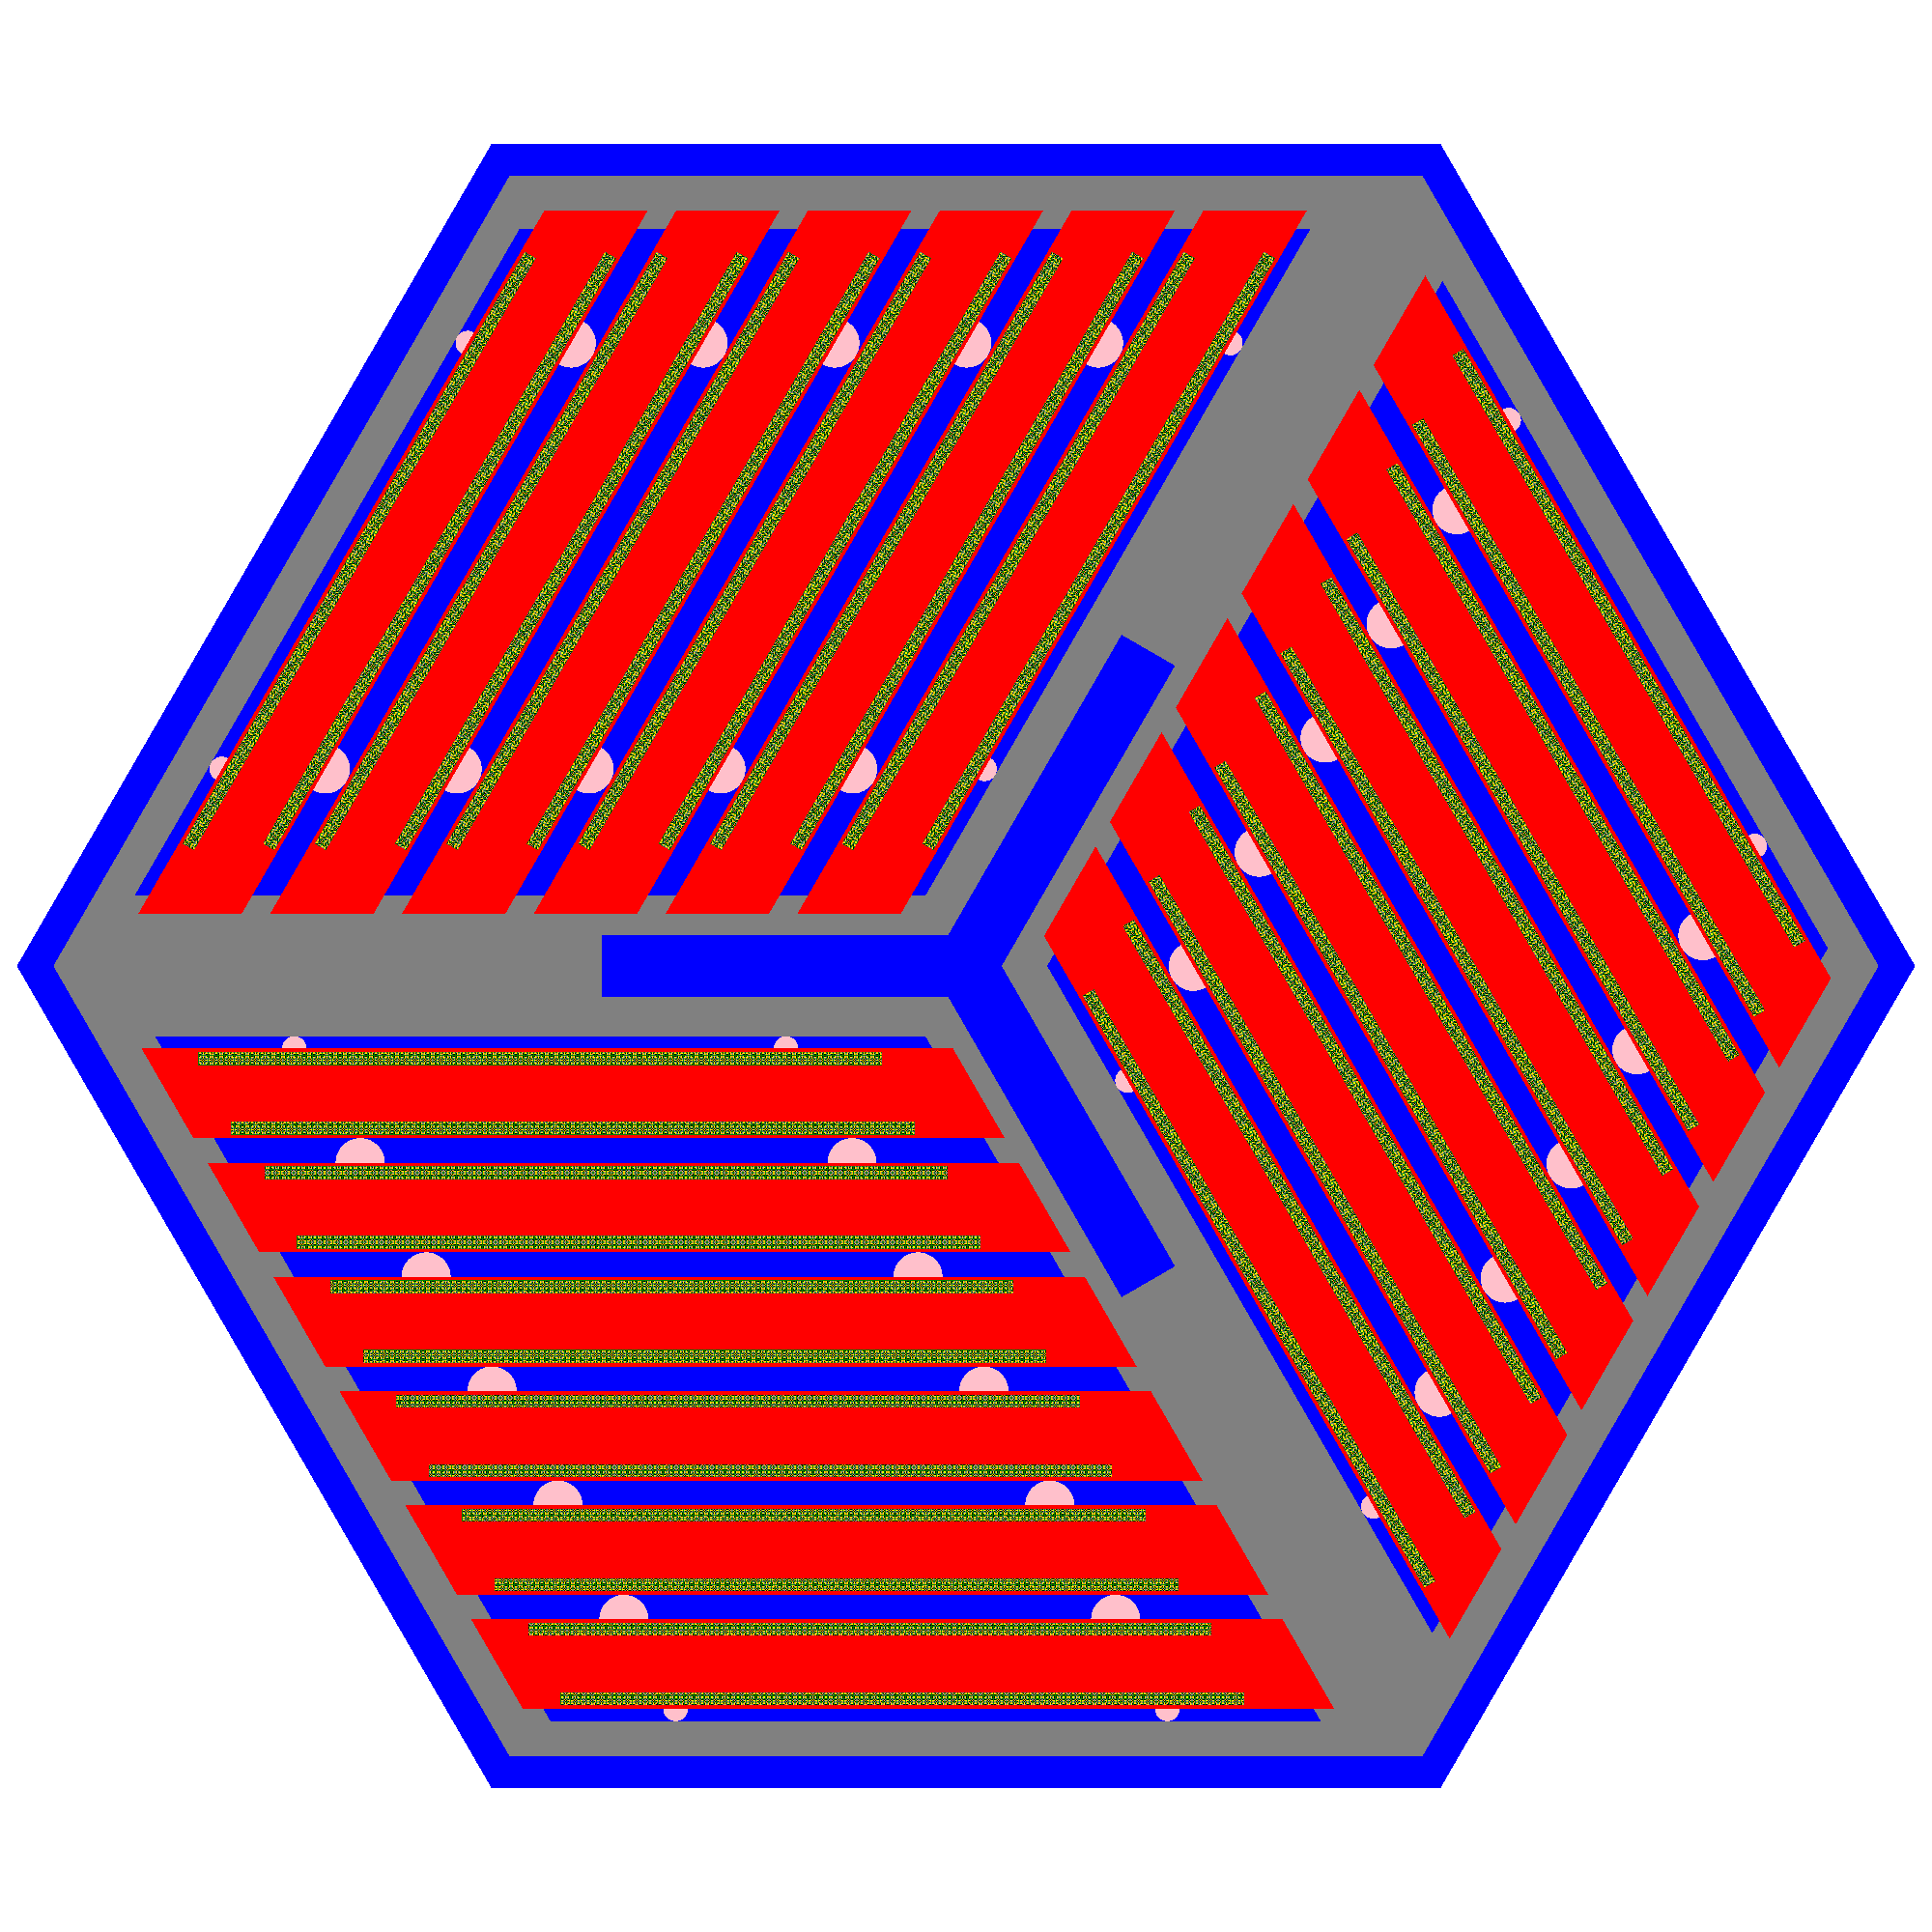
\includegraphics[width=0.5\linewidth]{ahtr-fuel-element.png} 
    \caption{FHR fuel element.}
    \label{fig:ahtr-fuel-element}
\end{figure}

The external channel wrapper and structural Y-shape as seen in Figure 
\ref{fig:y-shape} are made of C-C composite and have extra notches for the 
fuel plates to slide in. 
The gap between the fuel elements and fuel plates are filled with \gls{FLiBe}
coolant. 
At the center of the Y-shape structure is the Y-shaped control blade slot, 
which contains \gls{FLiBe} coolant when the control blade is not in the slot
\cite{varma_ahtr_2012,ramey_monte_2018,noauthor_fluoride_nodate}.

\begin{figure}[]
    \centering
    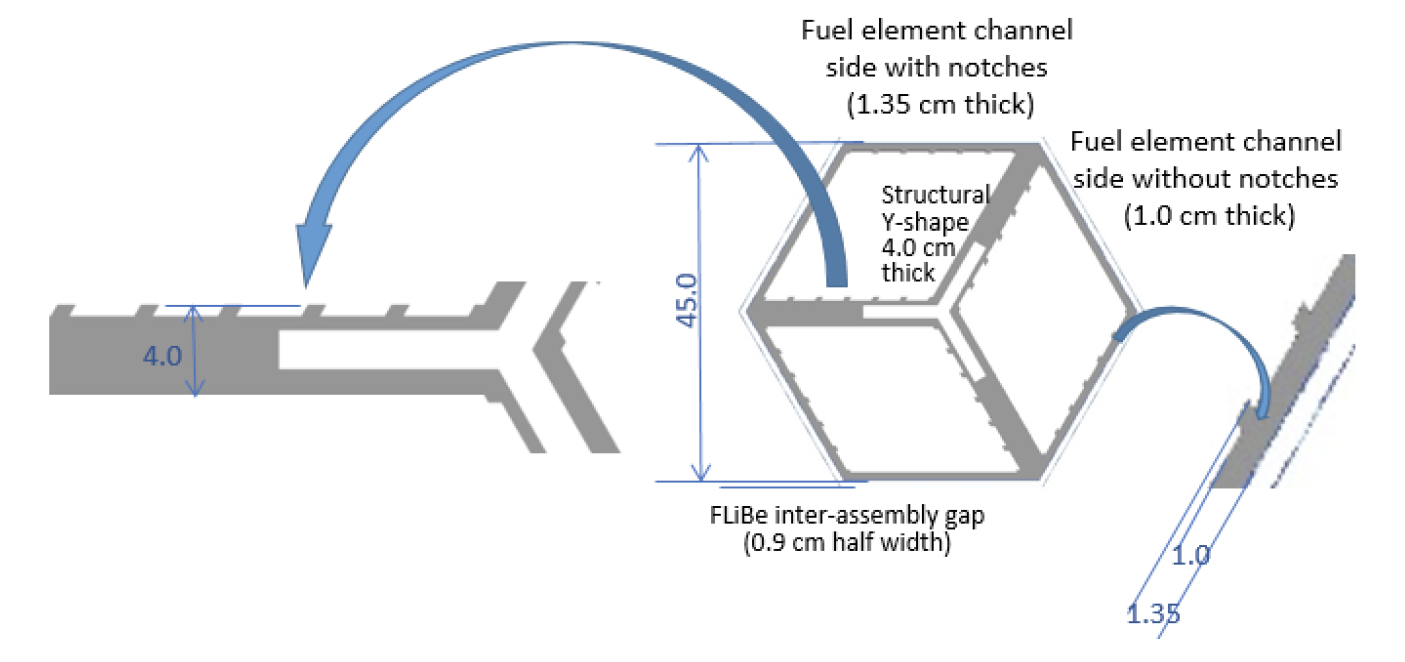
\includegraphics[width=0.8\linewidth]{y-shape.png} 
    \caption{FHR fuel element's structural components \cite{noauthor_fluoride_nodate}.}
    \label{fig:y-shape}
\end{figure}

Each fuel plank is made of an isostatically pressed carbon with fuel stripes 
on each outer side of the plank as seen in Figure \ref{fig:ahtr-fuel-plank}. 
The fuel stripes are prismatic regions composed of a graphite matrix filled with 
a cubic lattice of \gls{TRISO} particles. 
The lattice is 210 \gls{TRISO} particles wide in x-direction, 4 particles deep in 
the y-direction, and 5936 particles tall in the z-direction. 
Each \gls{TRISO} particle has 5 layers: Oxycarbide fuel kernel, porous carbon 
buffer, inner pyrolytic carbon, silicon carbide layer, and the outer pyrolitic 
carbon as seen in Figure \ref{fig:ahtr-triso}

\begin{figure}[]
    \centering
    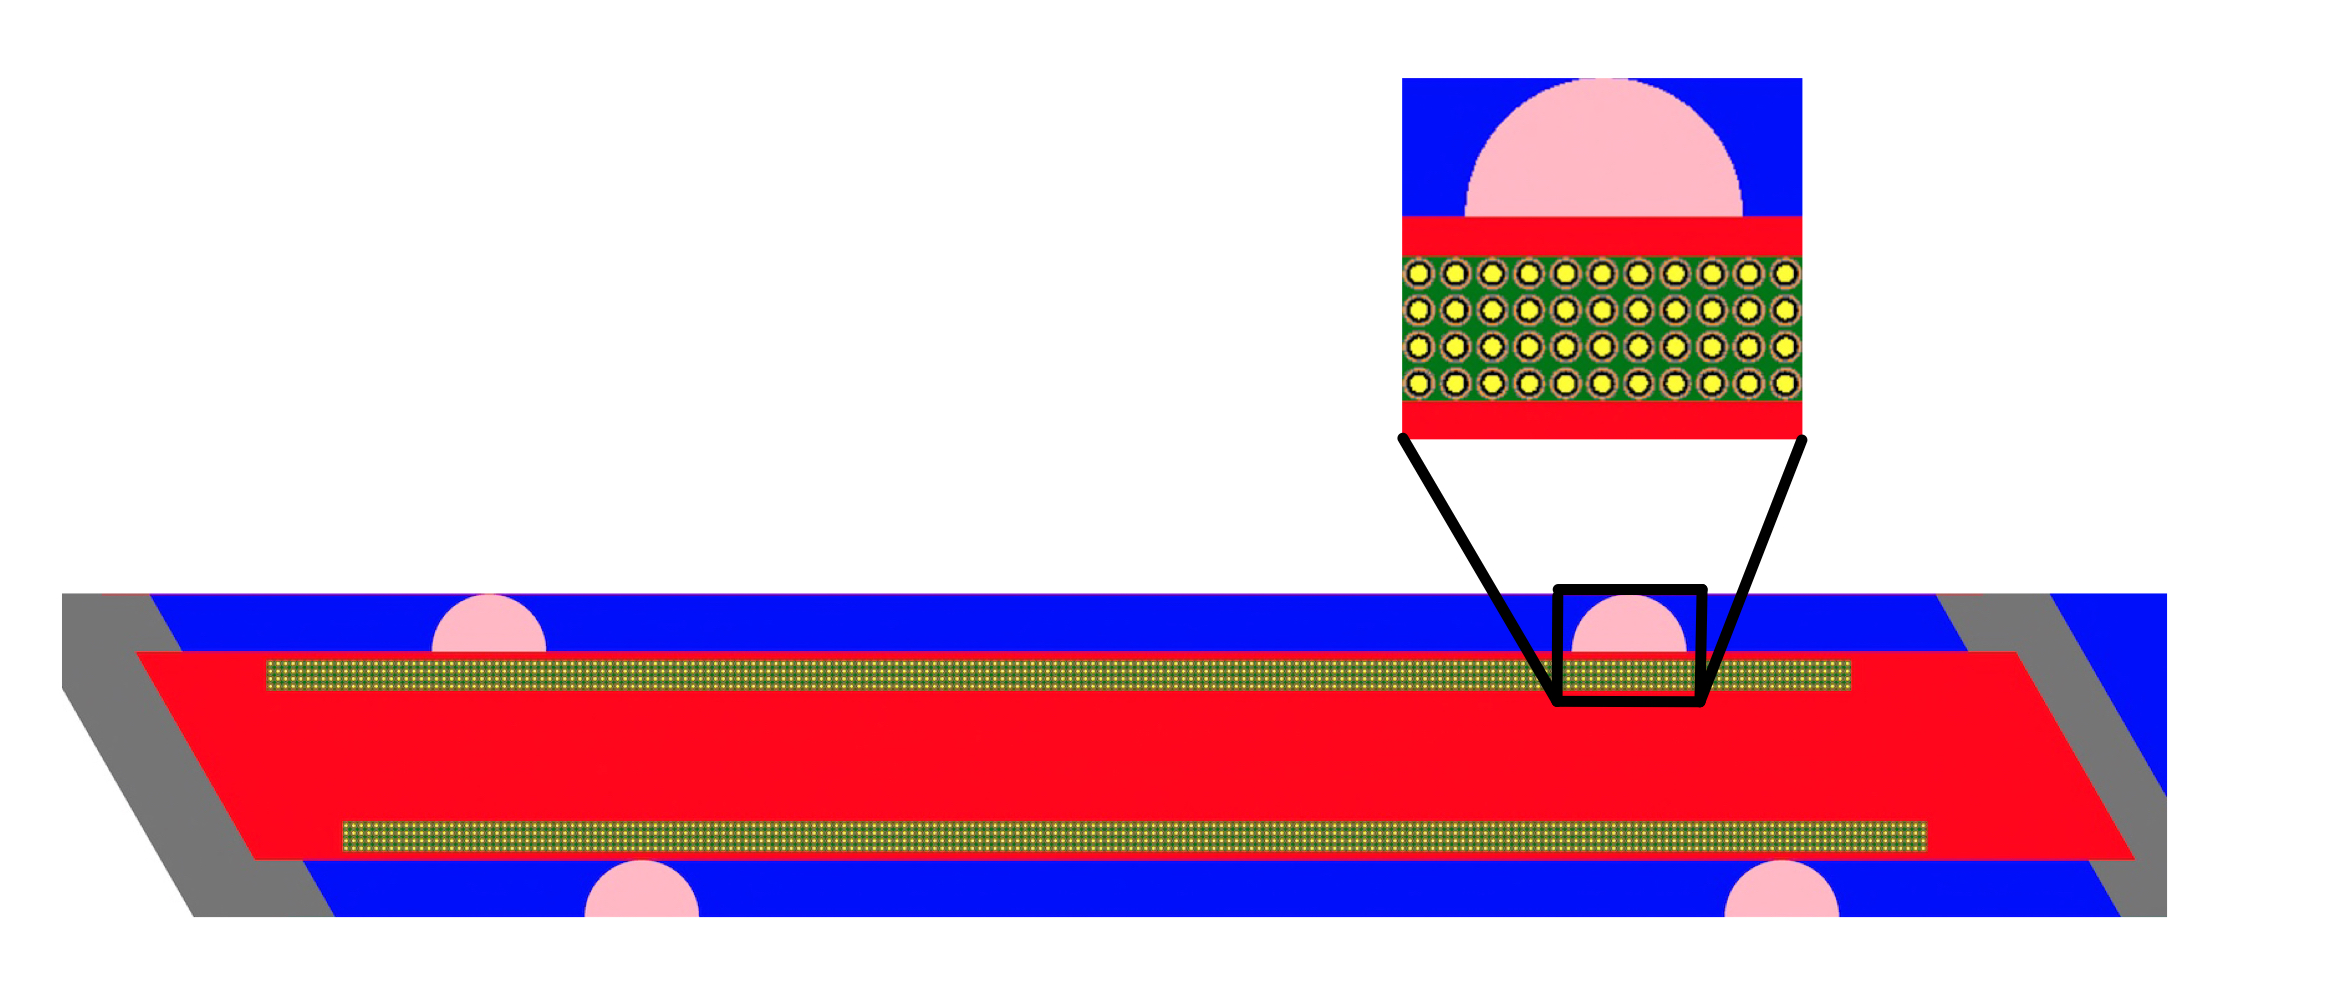
\includegraphics[width=0.8\linewidth]{ahtr-fuel-plank.png} 
    \caption{2D view of FHR fuel plank.}
    \label{fig:ahtr-fuel-plank}
\end{figure}

\begin{figure}[]
    \centering
    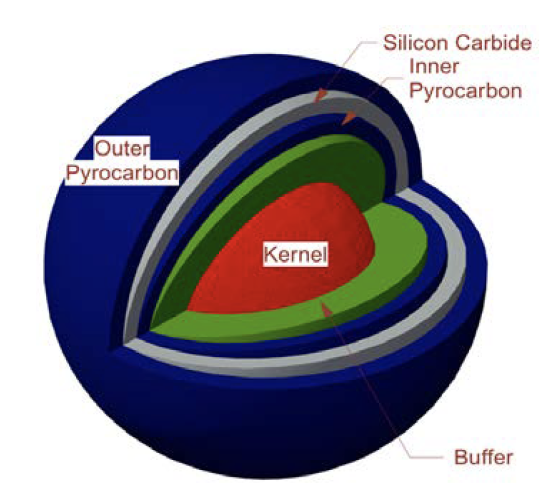
\includegraphics[width=0.4\linewidth]{ahtr-triso.png} 
    \caption{TRISO particle schematic \cite{noauthor_fluoride_nodate}.}
    \label{fig:ahtr-triso}
\end{figure}

\subsection{FHR Benchmark}


\section{Artificial Intelligence Applications to Nuclear Reactor Design}